
\chapter{Introduction and Motivation}
\label{Introduction} 

%1. Establishing your research territory
%2. Constructing the research gap or niche
%3. Pointing out the gap/niche
%4. Stating your purpose. Aim statement or research question
%5. Highlighting benefits and mapping out the paper


%1. Statements about the field of research
%to provide the reader with a setting or
%context for the problem to be
%investigated and claimed its centrality
%or importance.
%2. More specific statements about
%the aspects of the problem already
%studied by other researchers, laying
%a foundation of information already
%known.
%3. Statements that indicate the need for
%more investigation, creating a gap or
%research niche for the present study
%to fill.
%4. Statements giving the purpose/
%objectives of the writer's study or
%outlining its main activity or findings.
%5. Optional statement(s) that provide a
%positive value or justification for
%carrying out the study.

%\section{RISC-V and Open-source processors}

\section{Motivation}


With the end of Dennard scaling and the recent slowdown of Moore's Law, achieving performance and energy efficiency improvements from scaling down the transistors is becoming exponentially harder \cite{hennessyComputerArchitectureQuantitative2019}. This has led to a shift from general-purpose processor cores to \textit{\acrfull{dsa}}. Companies need to specialize their processors to achieve higher performance and lower energy instead of using an available general-purpose processor \cite{mezgerSurveyRISCVArchitecture2022}. 


The growing demand for specialized processors has also led to a demand for an open and modular \textit{Instruction Set Architecture (ISA)}. The RISC-V ISA \cite{watermanRISCVInstructionSet2019,watermanRISCVInstructionSet2021}, originally developed at UC Berkeley in 2010 \cite{pattersonComputerOrganizationDesign2021}, has recently gained popularity in academia and industry because of its open-source nature, proven RISC-style, and modularity \cite{theshdgroupRISCVMarketReport2024, asanovicInstructionSetsShould2014}.
The 2024 RISC-V Market Report by \textcite{theshdgroupRISCVMarketReport2024} reports 1.3B RISC-V units shipped in 2023 and forecasts growth to 16.2B units by 2030.


The RISC-V ISA consists of a base architecture with the possibility to add functionality through various extensions \cite{watermanRISCVInstructionSet2019}. This flexibility is particularly useful for \acrshort{dsa}s. It allows designers to start with a minimal processor, extend it with only the required extensions, and possibly add custom implementation-specific instructions. Custom extensions enable compute-intensive tasks to be implemented in hardware and accessed through custom instructions. 

Being an open-source ISA, anyone can use and modify RISC-V without a licensing fee. This allows a low barrier to entry and collaboration between developers and researchers. The open nature of RISC-V open-source ISA has also led to an increasingly large ecosystem of open-source processors. One such example is the CV32E40S \cite{openhwgroupCv32e40s2024}, a processor core from the CORE-V family of processor cores from the OpenHW Group, a global organization of many companies working together to make open-source cores, tools, and software \cite{taylorAdvancedRISCVVerification2023}. Mainly developed by Silicon Labs, the CV32E40S is a relatively small and efficient processor with a 4-stage pipeline. The core can be configured to support different RISC-V extensions and also adds the custom Xsecure extension, adding multiple security features \cite{openhwgroupIntroductionCOREVCV32E40S2023}. This processor will be used as an example throughout the thesis.





\subsection{Processor verification \& the need for a reference model}

Compared to trusted commercial solutions, the biggest barrier to adopting open-source processor cores in a System-on-Chip (SoC) is the processor core's quality, particularly the verification effort invested in the core. Compared to open-source software, hardware typically has a much higher manufacturing cost, increasing the verification requirements \cite{kevinmcdermottOpenHWIndustrialGradeVerification2022}.
With RISC-V, where "anyone" can make a processor, the verification responsibility is now moved from a few specialized IP suppliers to every SoC developer. 

Therefore, a versatile and open verification environment is essential to RISC-V's continuing popularity and growth. Verification is a crucial aspect of processor development, consuming a significant portion of the overall development time. If every developer team were to build their verification environment from scratch, the adoption of RISC-V would likely stagnate.

Conventional manual testing with predetermined outcomes can be time\--consuming and inadequate to thoroughly validate a processor's complex behavior. Instead, constrained random testing is often used to generate a wide range of test stimuli, covering many test cases. Variations of the "step-and-compare" methodology are widely utilized for processor verification \cite{taylorAdvancedRISCVVerification2023}. The diagram in \Cref{fig:testbench_block_diagram} shows an example of this, where the \acrfull{dut} processor core, written in \acrfull{rtl} code, runs in parallel with a golden \textit{\gls{rm}} written in a higher level language, all in a \acrfull{uvm} testbench environment. 

\begin{figure}
    \centering
    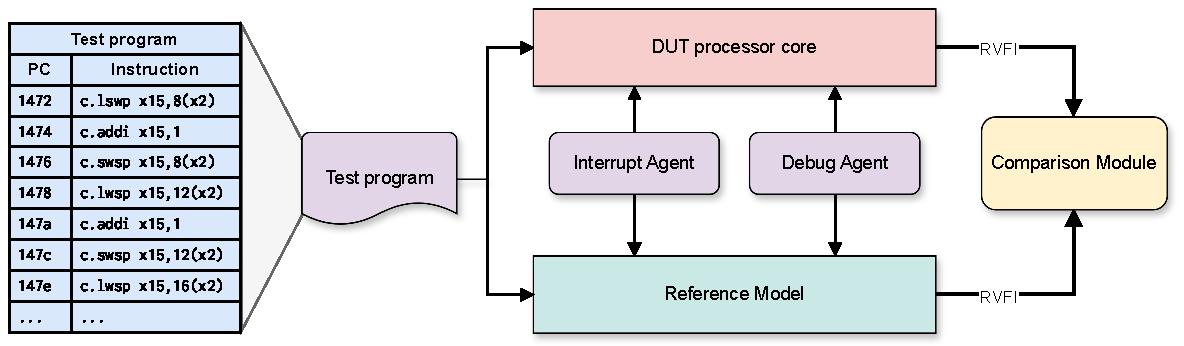
\includegraphics[width=1.00\linewidth]{figures/ISS_Testbench.pdf}
    \caption{Simple block diagram of a testbench with a reference model parallel to a processor core, running the same test program. }
    \label{fig:testbench_block_diagram}
\end{figure}


Throughout this thesis, we will define a \textit{Reference Model} as a high-level model of a processor used to verify the processor's implementation. An instruction\--accurate \textit{\acrfull{iss}} can be used as a reference model, but a reference model can also be a more advanced, cycle-accurate model. 

The \acrshort{dut} core and reference model run in lock-step, executing the same test program, one instruction at a time. 
The processor state of the core and reference model is usually compared after each instruction has been \textit{retired}, which is when the execution of the instruction has been completed, and all the state changes to registers and memory associated with the instructions have been updated \cite{taylorAdvancedRISCVVerification2023}. 

At the retirement of each instruction, the core and reference model outputs its state changes over the \textit{\acrfull{rvfi}}, which are compared by a comparison module. If a mismatch between the two is detected, this can be instantly flagged instead of running through the entire test program and comparing the results afterward. 

Asynchronous events, such as interrupts and debug requests, are injected into the core and reference module through \acrshort{uvm} agents, independently of the test program.

In RISC-V, the state of the processor is stored in multiple types of registers. The 32 \acrfull{gpr} are visible to the programmer, used for regular program execution, and are read from and written to by the instructions~\cite{watermanRISCVInstructionSet2019}. Additionally, the \acrfull{pc} is the register that holds the address of the current instruction \cite{watermanRISCVInstructionSet2019}. There is also a set of registers used to control and monitor the operation of the processor, called the \acrfull{csr}. 



\subsection{The challenge of verifying asynchronous events}

For verification of normal instruction execution, using an \acrfull{iss}, simulating the processor at the instruction level granularity is often sufficient. However, the ISS becomes inadequate when \textit{Asynchronous events}, interrupting the normal program flow, are introduced \cite{taylorAdvancedRISCVVerification2023}. They pose a challenge because of the differing abstraction levels of the ISS and the RTL code of the DUT, which can lead to improper timing of interrupts and \textit{side effects}. Asynchronous events in an ISS are synced to the beginning of an instruction, unlike in the RTL implementation, where asynchronous events can arrive at any cycle, and the timing can be affected by the state of the pipeline \cite{taylorAdvancedRISCVVerification2023}.


As a motivating example that we will come back to later, consider the two instruction traces in \Cref{fig:lw_example}. This shows the PC and instructions that the core and ISS run in a setup like \Cref{fig:testbench_block_diagram}, where we use an instruction-accurate ISS as the reference model. The figure shows that they will both correctly run the same instructions when they execute normal sequential code. The problem arises when an interrupt is injected into the core and ISS between PC \rv{1476} and \rv{1478}. Since the ISS fully completes its execution of an instruction before moving on to the next, the interrupt handler (in orange), starting at \rv{PC = 40}, is executed as the next instruction after the interrupt. In comparison, the core is modeled with a \textit{pipeline} that instructions move through over multiple clock cycles. The state of the pipeline can give a delay where the interrupt cannot be taken immediately, causing more instructions to be retired in the core before the interrupt is taken. 

\begin{figure}
    \centering
    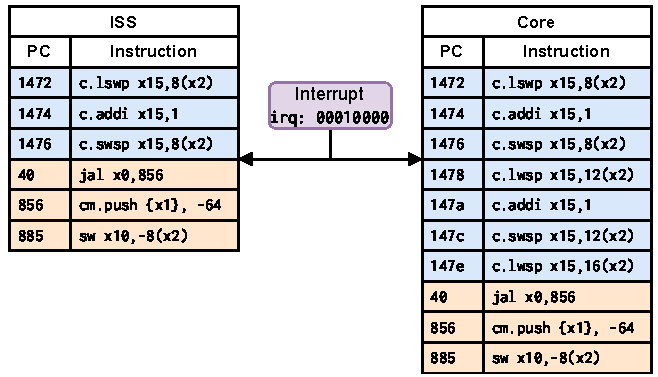
\includegraphics[width=0.75\linewidth]{figures/lw_add_sw_example.pdf}
    \caption{Simple example showing interrupt injection into an ISS and a core.}
    \label{fig:lw_example}
\end{figure}



Correctly predicting the delay between the interrupt injection and when the interrupt is taken is one of the major problems with this verification strategy. The delay is highly dependent on core-specific functionality and cycle-accurate timing, making this delay hard to predict \cite{taylorAdvancedRISCVVerification2023}. 

The problem above becomes even more complicated when multiple different asynchronous events are triggered concurrently, as core-specific functionality affects how these events influence each other, which event will be taken first, and how this affects the timing. 






%\begin{terminal}
%c.li x11,0
%c.addi x11,1
%c.addi x11,2
%c.addi x11,3
%c.addi x11,4
%c.addi x11,5
%
%c.lwsp x15,8(x2)
%c.addi x15,1
%c.swsp x15,8(x2)
%c.lwsp x15,12(x2)
%c.addi x15,1
%c.swsp x15,12(x2)
%c.lwsp x15,16(x2)
%\end{terminal}


%\section{Approach/scope of the report}

%
%


%\section{Requirements}
%\begin{itemize}
%    \item Cycle-level simulation
%    \item Run in async lock-step-compare with openHW core (e.g. CV32E40S)
%    \item Handle async events
%    \item handle hardware real-time effects
%    \item Pipeline understanding
%    
%\end{itemize}

\section{Objectives}




In this thesis, we aim to design and implement a reference model for RISC-V processors that can accurately simulate asynchronous events such as interrupts and debug requests. It builds upon the conclusions from the author's previous specialization project \cite{torjenygaardeikenesDesigningRISCVReference2023} that explored different approaches for designing a cycle-accurate reference model. 
The project concluded that a two-layered reference model with a \textit{pipeline shell} on top of an existing ISS could be a promising solution. 

We will further explore this two-layered approach by designing, implementing, and verifying it. The goal is to determine whether the approach can improve the verification of RISC-V processors, particularly in handling asynchronous events. 

We also want to determine if this approach can work with formal verification and how the design can be useful for different processor cores.


\section{Research Methodology}

We will explore an architecture where the "untimed" ISS is responsible for the functional execution of instructions while the pipeline shell is responsible for correctly timing these instructions and controlling the timing of asynchronous events. We will also focus on how the reference model can easily be modified to different processor cores and if it can be compatible with formal verification.  
To achieve this, we will cover the following points:
\begin{raggedright}
\begin{enumerate}
    \item Highlight the complexities of verifying asynchronous events. 
    \item Discuss the shortcomings of existing solutions.
    \item Design, architect, and implement a reference model to simulate asynchronous events correctly. We will start with a simple model and later expand it to support asynchronous events and the pipeline shell.
    \item Verify the correctness of the model by comparing the execution to the CV32E40S core, treating this as a golden model.
    \item Compare the solution to previous solutions.
    \item Evaluate whether the reference model is compatible with formal verification.
    \item Discuss the viability of the proposed solution.
\end{enumerate}
\end{raggedright}

%To achieve this, we will first implement a simple reference model resembling a traditional ISS before adding the asynchronous events and the pipeline shell. To verify its correctness, we will compare the execution of the reference model to the CV32E40S core, using this core as a golden model. We will also compare the solution to previous solutions and evaluate whether the reference model is compatible with formal verification.


%\tmp{Hvilke spørsmål ønsker jeg å finne svar på og hva vil jeg løse gjennom arbeidet}


\section{Contributions}

The most important contributions of this thesis are:

\begin{enumerate}
    \item Implementing a reference model with a pipeline shell around Spike.
    \item Expanding the Spike ISS to support traditional simulation of the CV32E40S core.
    \item Modifying the Spike ISS to work with the proposed reference model solution, enhancing RVFI support, injecting interrupts and debugging requests, and state reversion.
    \item Adding Onespin support to the core-v-verif environment to enable formal verification of the CV32E40S core.
\end{enumerate}

These contributions have been merged into the core-v-verif Github Repository~\cite{openhwgroupOpenhwgroupCorevverif2023}.


\section{Outline}


\begin{itemize}
    \item \textbf{\Cref{ch:Background}: \nameref{ch:Background}} provides background information on pipelining, interrupts, debug requests, processor verification techniques, Instruction Set Simulators (ISS), existing RISC-V reference model solutions, the CV32E40S verification environment, the challenges of using an ISS as a reference model, and cycle-accurate modeling techniques.
    
    \item \textbf{\Cref{ch:specialization}: \nameref{ch:specialization}}  
    summarizes the author's previous work on this topic, highlighting the key findings and conclusions from the previous specialization project. %This chapter serves as a starting point for the current research and identifies areas for further exploration.
    
    \item \textbf{\Cref{ch:design}: \nameref{ch:design}} 
    outlines the design requirements for the reference model and discusses the architectural choices made to meet these requirements. It covers the overall architecture, choice of implementation language, interface design, partitioning of tasks between the ISS and pipeline shell, and considerations for formal verification. The requirements proposed here influence the similar requirements in \Cref{ch:PipelineShell} and \Cref{ch:ISS}.
    
    \item \textbf{\Cref{ch:PipelineShell}: \nameref{ch:PipelineShell}}  
    provides a detailed explanation of the pipeline shell implementation. It covers the requirements, architecture, interaction with the ISS, dependency on the core, pipeline stage modeling, controller module design, and handling asynchronous events.% instruction stepping, interrupt handling, timing of side effects, flushing, state reversion, and handling of other asynchronous events.
    
    \item \textbf{\Cref{ch:ISS}: \nameref{ch:ISS}} 
    focuses on the Instruction Set Simulator (ISS) used in the reference model. It discusses the ISS requirements, the rationale behind choosing Spike, and the modifications to integrate it with the reference model, including injecting interrupts and debug requests and reverting the state.
    
    \item \textbf{\Cref{ch:formal}: \nameref{ch:formal}} covers the contribution of adding support for the Onespin tool for formal verification and how the reference model can be verified using formal verification.
    
    
    \item \textbf{\Cref{ch:results}: \nameref{ch:results}}
    presents the results of the tests, compares the design to previous reference model solutions, and discusses the strengths and weaknesses of the implemented reference model.
    
    \item \textbf{\Cref{ch:conclusion}: \nameref{ch:conclusion}} 
    concludes the thesis and proposes future work.
\end{itemize}

%\begin{figure}
%    \centering
%    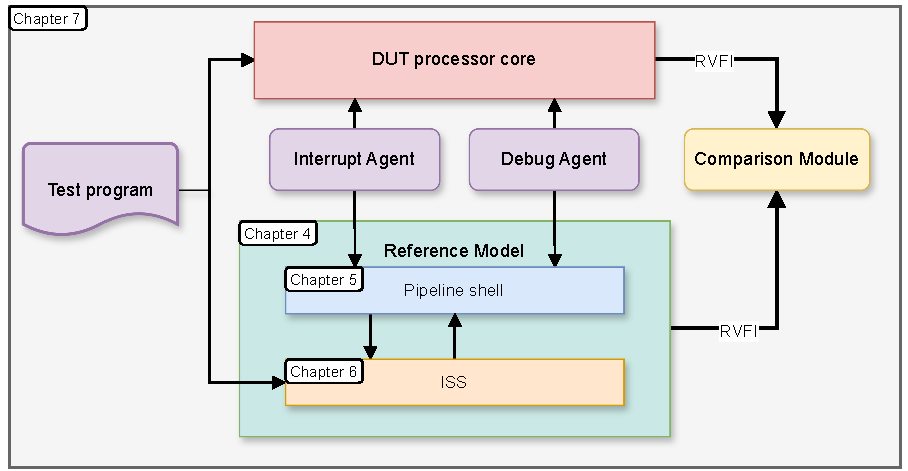
\includegraphics[width=0.75\linewidth]{figures/architecture_outline.pdf}
%    \caption{\tmp{Bør jeg ha med denne?} \tmp{TODO: Fiks kapittelnummer}Block diagram of the Reference Model and surounding components, and which chapter these will be discussed.}
%    \label{fig:block-outline}
%\end{figure}

%\Cref{ch:Background} will describe how interrupts are handled in RISC-V and how they are affected by the pipeline. We will also describe common verification techniques and verification environments, and introduce different Instruction Set Simulators.
%
%\Cref{ch:Reference Model} will discuss the design and architecture of a reference model featuring a pipeline shell modeled around an existing ISS. We will compare different pipeline shell implementations, existing ISSs, and interfaces between the pipeline shell and the ISS. The CV32E40X core from the OpenHW Group will be used as an example processor to model. Still, we will also consider how the reference model can be easily configurable to different cores.
%

